\documentclass[tikz,border=5pt]{standalone}
\usepackage{tikz}
\usepackage{amsmath}

\begin{document}

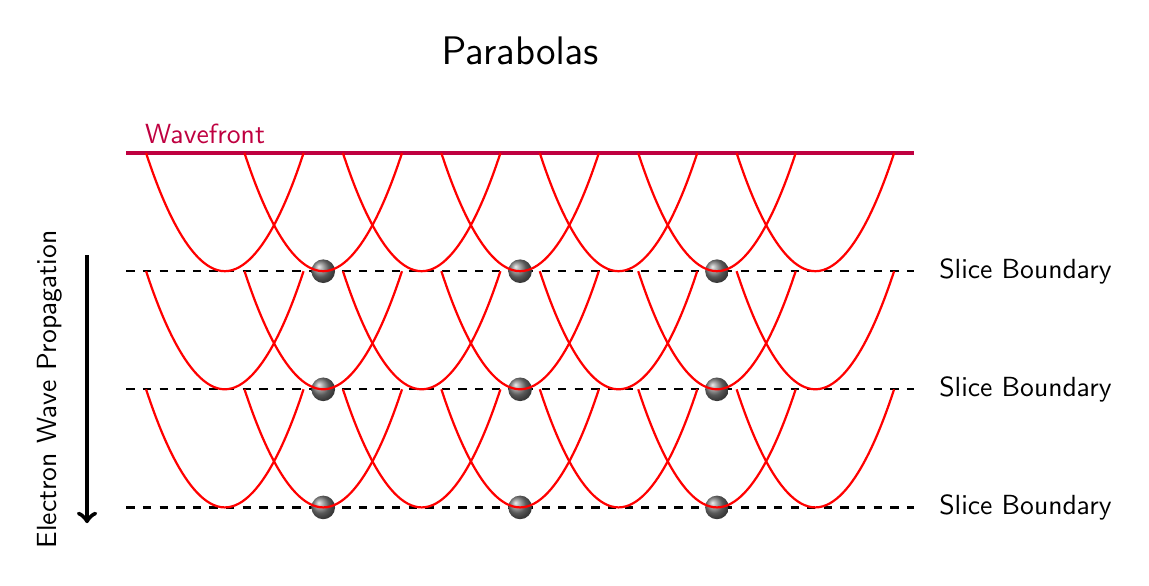
\begin{tikzpicture}[font=\sffamily]
    % Define coordinates for the planes
    \coordinate (TopPlaneLeft) at (0, 3);
    \coordinate (TopPlaneRight) at (10, 3);
    \coordinate (MidPlaneLeft) at (0, 1.5);
    \coordinate (MidPlaneRight) at (10, 1.5);
    \coordinate (BotPlaneLeft) at (0, 0);
    \coordinate (BotPlaneRight) at (10, 0);

    % Title
    \node[anchor=south] at (5, 5.5) {\Large Parabolas};

    % Draw Atomic Planes and Atoms
    \foreach \y in {0, 1.5, 3} {
        \draw[thick, black, dashed] (0,\y) -- (10,\y);
        \node[anchor=west] at (10.2, \y) {Slice Boundary};
        % Only 3 atoms spaced out
        \foreach \x in {2.5, 5, 7.5} {
            \shade[ball color=gray] (\x, \y) circle (0.15);
        }
    }

    % Electron Wave Propagation Arrow
    \draw[->, ultra thick, black] (-0.5, 3.2) -- (-0.5, -0.2);
    \node[rotate=90, anchor=south, black] at (-0.7, 1.5) {Electron Wave Propagation};
    
    % Wavefront line
    \draw[ultra thick, purple] (0, 4.5) -- (10, 4.5);
    \node[purple, anchor=south] at (1, 4.5) {Wavefront};

    % Fresnel Propagation Parabolas
    
    % Parabolas landing on the Wavefront from above have been removed.

    % 1. Parabolas between Wavefront (y=4.5) and Top Plane (y=3)
    % Increased density
    \foreach \x in {1.25, 2.5, 3.75, 5, 6.25, 7.5, 8.75} {
         \draw[thick, red] (\x-1, 4.5) parabola bend (\x, 3) (\x+1, 4.5);
    }
    
    % 2. Parabolas between Top Plane (y=3) and Middle Plane (y=1.5)
    \foreach \x in {1.25, 2.5, 3.75, 5, 6.25, 7.5, 8.75} {
         \draw[thick, red] (\x-1, 3) parabola bend (\x, 1.5) (\x+1, 3);
    }
    
    % 3. Parabolas between Middle Plane (y=1.5) and Bottom Plane (y=0)
    \foreach \x in {1.25, 2.5, 3.75, 5, 6.25, 7.5, 8.75} {
         \draw[thick, red] (\x-1, 1.5) parabola bend (\x, 0) (\x+1, 1.5);
    }

\end{tikzpicture}

\end{document}
